% chapter massa_and_movoir (fold)
\chapter{Enhancing \massa{} to support VO datasets}
\label{cha:massa_and_movoir}
	
	In chapter \ref{cha:using_legacy_tools} we discussed what
	constitutes a VO application, and we reached the
	conclusion that a VO application could be one that
	supported VO application messaging, and VO file formats.
	Such an application could rely on existing VO Data Access
	modules, and share the data products it creates with
	other tools.
	
	Besides, in chapter~\ref{cha:movoir} we further discussed what
	kind of messages should be implemented by MOVOIR applications,
	and saw two different kind of messages:
	
	\begin{description}
		\item[Standard VO data interchange messages] These
		are messages from the standard suite of SAMP MTypes,
		that is, those shown on
		section~\ref{sec:already_defined_mtypes}.
		
		\item[MOVOIR specific messages] We can further divide
		this kind of messages into:
		
		\begin{description}
			\item[Self-description messages] Those used in order
			to provide a self-dis\-cov\-e\-ry, and self-description
			API which can be used by automated tools in order
			to create appropriate messages. These were proposed
			in section~\ref{sec:describing_mtype_parameters}.
			
			\item[Function messages] These are messages created
			for implementing direct access to the functionality
			offered by a MOVOIR module.
		\end{description}
	\end{description}
	
	We further established in section~\ref{sec:movoir_modules} 
	which should be the modules needed in order to be able to
	provide a complete VO environment for legacy applications:
	
	\begin{description}
		\item[VO Downloader] Application to enable the download
		of VOTables and FITS files, using \method{table.load.*}
		and \method{image.load.fits} messages.
		
		\item[VOTable to FITS converter] Similar to the VO
		Downloader, the VOTable converter is an application
		which creates FITS files from \method{ta\-ble.load.vo\-ta\-ble}
		messages, saving the converted FITS file.
		
		\item[VO Registry and DAL module] This module is left
		to already existing applications, such as the VO~Desktop.
	\end{description}

	In addition, two more modules can be created to show the
	flexibility of the MOVOIR framework:
	
	\begin{description}
		\item[AMIGA ConeSearch module] This module is an
		example for using the 
		\method{co\-ord.point\-At.sky} MType to send back as a
		\method{table.load.votable} message the results
		of a ConeSearch of a fixed radius around the
		\mapkey{ra} and \mapkey{dec} coordinates obtained by
		clicking on an image with a World Coordinate System set
		on applications supporting both sending
		\method{co\-ord.point\-At.sky} and receiving 
		\method{table.load.votable}.

		\item[Sesame query module] This module is an example of
		a non-standard MType supporting module, so that MOVOIR
		provides a multi-object Sesame query message, as support
		for a future multi-cone search service, which can
		resolve multiple objects at once.
	\end{description}
	
	In this chapter, we will show how we have built each of
	these modules, and which have been the key points to take
	into account during the implementation for each of them,
	with the final goal of incorporating \massa{} into the VO.
	
	\section{VO Downloader} % (fold)
	\label{sec:vo_downloader}
		\newcommand{\downloadmgrurl}
		{http://www.sourcecodesworld.com/source/show.asp?ScriptId=1185}
		In order to create the VO~Downloader, we started with the
		source code for a simple Java-based URL downloader
		application\urlnote{\downloadmgrurl}, consisting of only 4
		classes: the DownloadManager class represents the main View
		and Controller classes; the Download class is the threaded
		Controller and Model for each actual download;
		the DownloadTableModel class is the Model for the Table
		View in DownloadManager; and DownloadProgressRenderer is a
		delegate class for the renderer sub-view.
		
		In order to be able to download files sent from any
		application, the VO~Downloader needs to respond to all data load messages ---\method{ta\-ble.load.vo\-ta\-ble},
		\method{ta\-ble.load.fits}, and \method{im\-age.load.fits}---
		In addition, a generic \method{movoir.download.file} is
		supported, plus the \method{mo\-vo\-ir.de\-scribe.m\-type}
		MType.
		
		\subsection{Implementation details} % (fold)
		\label{sub:implementation_details_vodownloader}
			
			\newcommand{\initSamp}
			{\method{initSamp()}}
			\newcommand{\shutdownSamp}
			{\method{shutdownSamp()}}
			
			As the VO~Downloader is a Java application, we will
			use the JSAMP\urlnote{\jsampurl} Java-based SAMP
			toolkit in order to implement JSAMP support.
			
			In
	section~\ref{sec:implementing_samp_into_an_existing_application}
			we indicated that, in principle, the changes to an
			existing application for the application to incorporate
			SAMP were minor, and were restricted to application
			setup, application shutdown, and the creation of the
			handlers for SAMP messages. We will show that in
			VO~Downloader, and the solution is exactly the same for
			\massa{}.
			
			\begin{figure}[tbp]
				\centering
					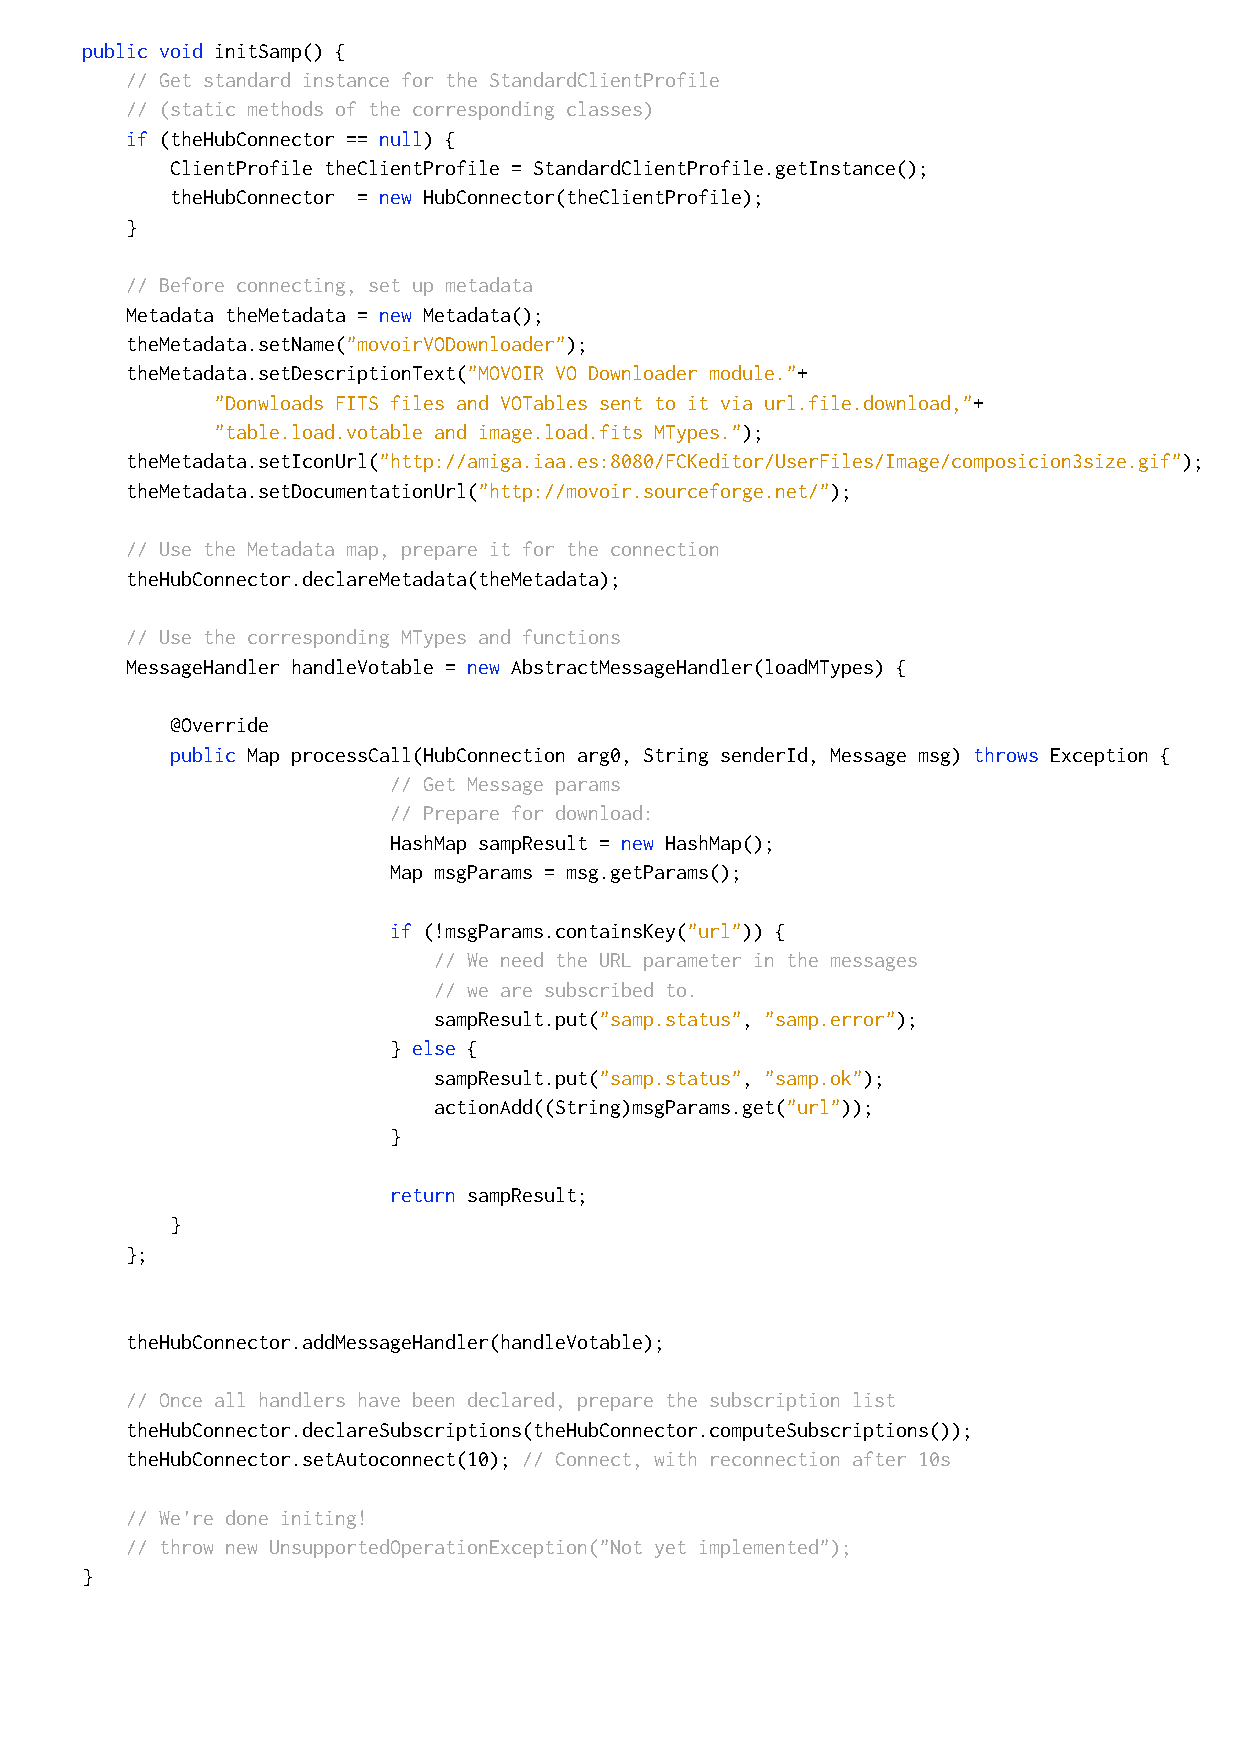
\includegraphics[width=\textwidth]
					{fig/VODownloader_initSamp.pdf}
				\caption[VO Downloader: \texttt{initSamp()}]
				{
					Section of VO~Downloader source code:
					\initSamp{} function, last in the
					VO~Downloader creator.
				}
				\label{fig:fig_VODownloader_initSamp}
			\end{figure}
			
			Figure~\ref{fig:fig_VODownloader_initSamp} shows the
			\initSamp{} function, which performs the
			initialisation of the SAMP messaging module within
			VO~Downloader. \initSamp{} is the last call in
			the VO~Downloader creator of the DownloadManager.
			
			The MOVOIR VO~Downloader interface is show in 
			figure~\ref{fig:fig_VODownloader}, while the
			VO~Downloader detail in the JSAMP HubMonitor can be
			seen in figure~\ref{fig:fig_Hub_topcat_vodownloader}.
			
			\begin{figure}[tbp]
				\centering
					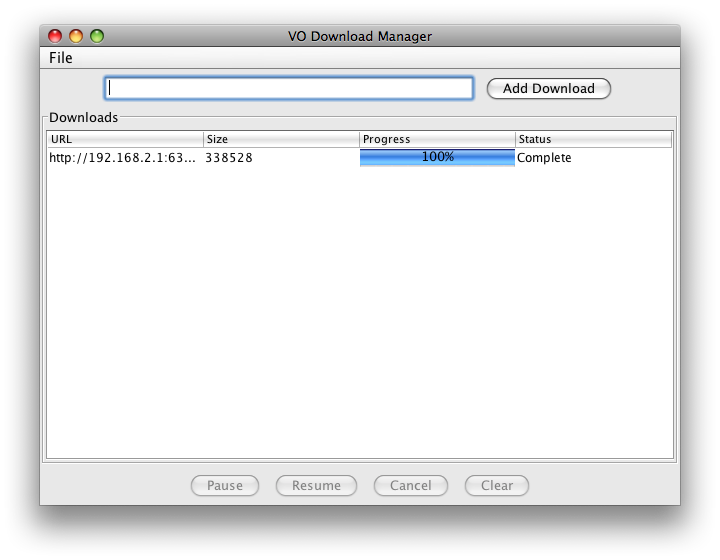
\includegraphics[height=0.4\textheight]
					{fig/VODownloader.png}
				\caption[VO Downloader receiving a VOTable]
				{
					VO~Downloader, with one download complete after
					receiving a \method{table.load.votable} from
					TOPCAT.
				}
				\label{fig:fig_VODownloader}
			\end{figure}
			
			\begin{figure}[tbp]
				\centering
					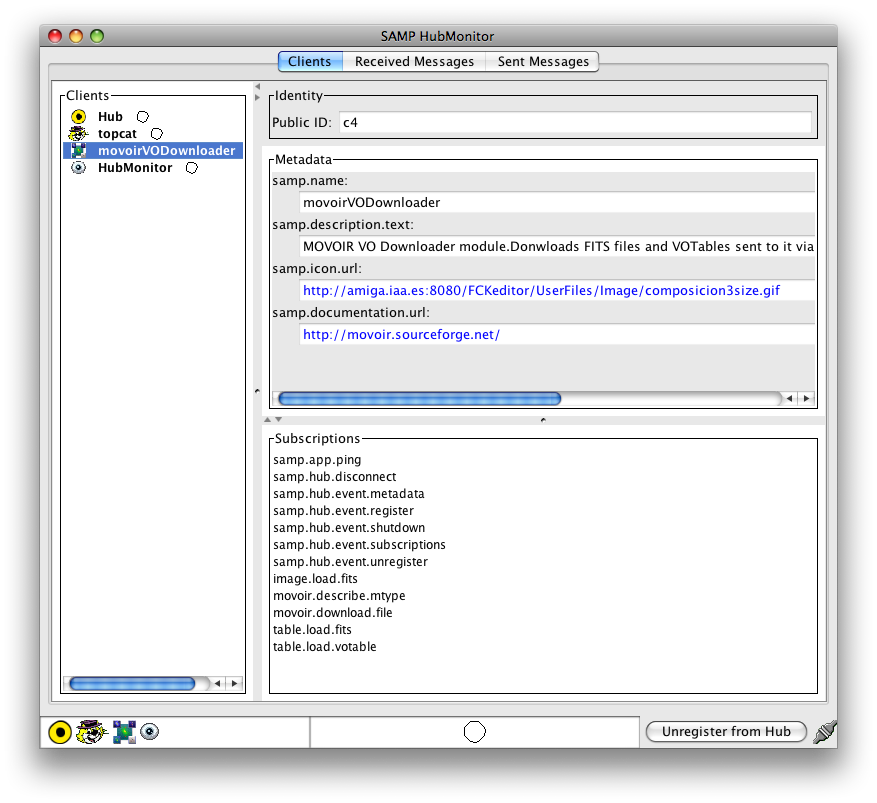
\includegraphics[height=0.4\textheight]
					{fig/Hub_topcat_vodownloader.png}
				\caption[VO Downloader in the JSAMP Hub Monitor]
				{JSAMP Hub Monitor showing the
				supported messages of the VO~Downloader}
				\label{fig:fig_Hub_topcat_vodownloader}
			\end{figure}
			
			 We can see that \initSamp{} provides an
			abstract SAMP message handler,
			\method{handle\-Vo\-ta\-ble()}, which receives three
			parameters:
			
			\begin{description}
				\item[\method{HubConnection hubConnect}] This
				parameter holds an instance of the JSAMP
				\method{Hub\-Con\-nec\-tion} class, and is profile
				specific. In the case of the SAMP standard profile,
				this parameter holds the details for connecting to
				the hub via XML-RPC.
				
				 \item[\method{String senderId}] This parameter
				provides a string with the unique identifier of the
				application that sent (or broadcasted) a message to
				our handler. We will use this in order to create
				messages back to the sender with the result of our
				computations. In the case of VO~Downloader, the
				results is always a \sampok{} answer, or a
				\samperror{} if the message does not provide a
				\method{url} parameter within the \sampparams{}
				map.
				
				 \item[\method{Message msg}] The \method{msg}
				parameter is the map described in
				section~\ref{sec:samp_messages_mtypes}, and
				provides all the actual message information:
				\sampmtype{}, for choosing the function to be
				performed, and \sampparams{} for the function to
				work.
			\end{description}
			
			In the case of VO~Downloader, the messages which are
			implemented are \method{ta\-ble.load.vo\-ta\-ble},
			\method{im\-age.load.fits}, \method{ta\-ble.load.fits}, and
			the MOVOIR-specific \method{movoir.download.file}
			(passed as a list of MType strings in
			\method{load\-M\-Types}). All of those messages need to
			provide a \mapkey{url} parameter.
			
			 If \mapkey{url} is present, the already implemented
			\method{actionAdd(String
			url\-String)} method is called in order to queue the
			download of the corresponding data. We can see that the
			\method{actionAdd} method already existed in
			VO~Downloader, and our handler just delegates the actual
			behaviour to an already existing function.
			
			 An additional \shutdownSamp{} method is called
			from the \method{actionExit()} method. Following the
			flow diagram shown in
			figure~\ref{fig:fig_SAMPEnabledAppFlow}, we have just
			modified:
			
			\begin{description}
				\item[VO~Downloader creator] We have added an
				\method{initSamp} method to declare the messages we
				are prepared to handle, at the end of the creator
				of the DownloadManager class of the VO~Downloader.
				
				 \item[Event handling] The event handling is
				modified by the same \method{initSamp} method, by
				adding listeners to SAMP messages with the
				\method{addMessageHandler} method. The message
				handler uses existing controller methods to
				delegate the actual implementation of the handler.
				
				 \item[VO~Downloader shutdown] In the case of the
				VO~Downloader, the original DownloadManager shutdown
				is handled by the the \method{actionExit} method,
				and the shutdown of the SAMP messaging in
				VO~Downloader is implemented as the first function
				in that method. For other applications, equivalent
				placements, if possible within a guaranteed
				execution thread, need to be chosen.
			\end{description}
			
			In order to implement the
			\method{movoir.describe.mtype} method, the easiest way
			is to create a separate handler (to be added with
			\method{addMessageHandler} of the \method{HubConnector}
			class), that use statically created maps. However, it
			is simpler, and more illustrative to create the result
			map within the handler itself.
			Figure~\ref{fig:fig_handleMovoirDescribe} shows the
			listing of the \method{movoir.describe.mtype} method
			handler supporting just the \method{table.load.votable}
			MType.
			
			\begin{figure}[tbp]
				\centering
					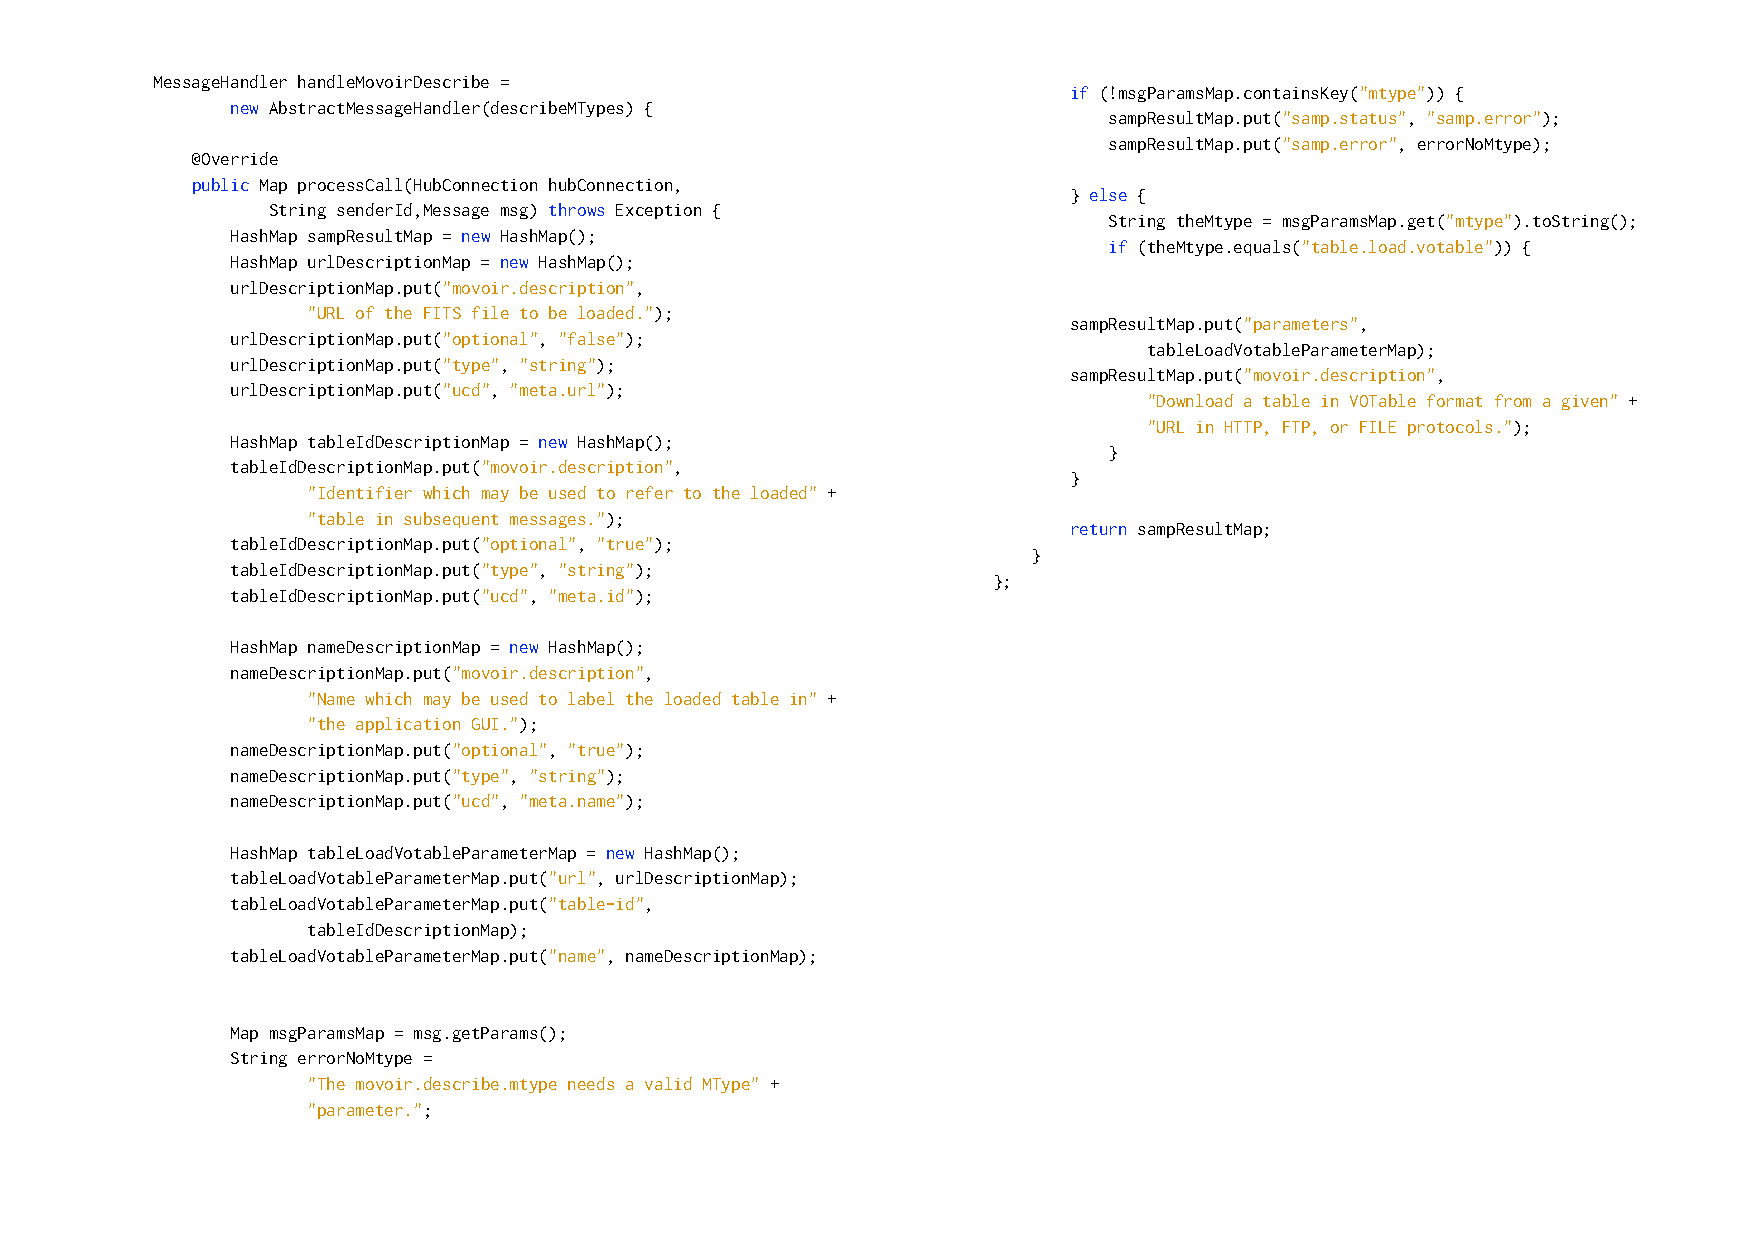
\includegraphics[width=\textwidth]
					{fig/handleMovoirDescribe.pdf}
				\caption[
					Handler of the \method{movoir.describe.mtype}
					message.
				]
				{
					Partial listing of the
					\method{movoir.describe.mtype} SAMP message
					handler, with the response map created on the
					fly.
				}
				\label{fig:fig_handleMovoirDescribe}
			\end{figure}
			
			
		% subsection implementation_details_vodownloader (end)
			
	% section vo_downloader (end)
	
	\section{VO Data Converter} % (fold)
	\label{sec:vo_data_converter}
		
		The VO Data Converter is another MOVOIR
		module needed to support those legacy applications for which
		source code is not available. As legacy applications
		will usually provide zero support for VOTables, data sent
		to the VO Data Converter will only be directly useful for
		legacy applications in FITS or ASCII formats.
		
		But in order to simplify that process, and eliminating
		the conversion step after download, we will create two
		separate VO Data Converters: one that converts VO tables
		into FITS tables, and another one which converts VO tables
		into CSV files.
		
		\subsection{Implementation details} % (fold)
		\label{sub:implementation_details_vodc}
		
			As only VOTables will need to be converted (FITS files
			are usually supported by legacy applications), those two
			modules need to be subscribed just to the
			\method{table.load.votable} MType. The response they
			need to provide to that message is the conversion to
			to the corresponding data format.
			
			We will write both modules (which will be quite similar)
			in Python, using the
			SAMPy\urlnote{\sampyurl} module developed by Luigi
			Paioro. They will also make use of the
			STILTS\urlnote{\stiltsurl}, by Mark Taylor, called as a
			command line tool from the Python scripts, which will also
			make use of the \method{curl} command for consolidating the
			download of the URL parameter.
			
			By using a different language we are also validating the
			multi-language support of the MOVOIR, which allows to use
			the language which provides the most ease of implementation
			for each module.
			
			\begin{figure}[tbp]
				\centering
					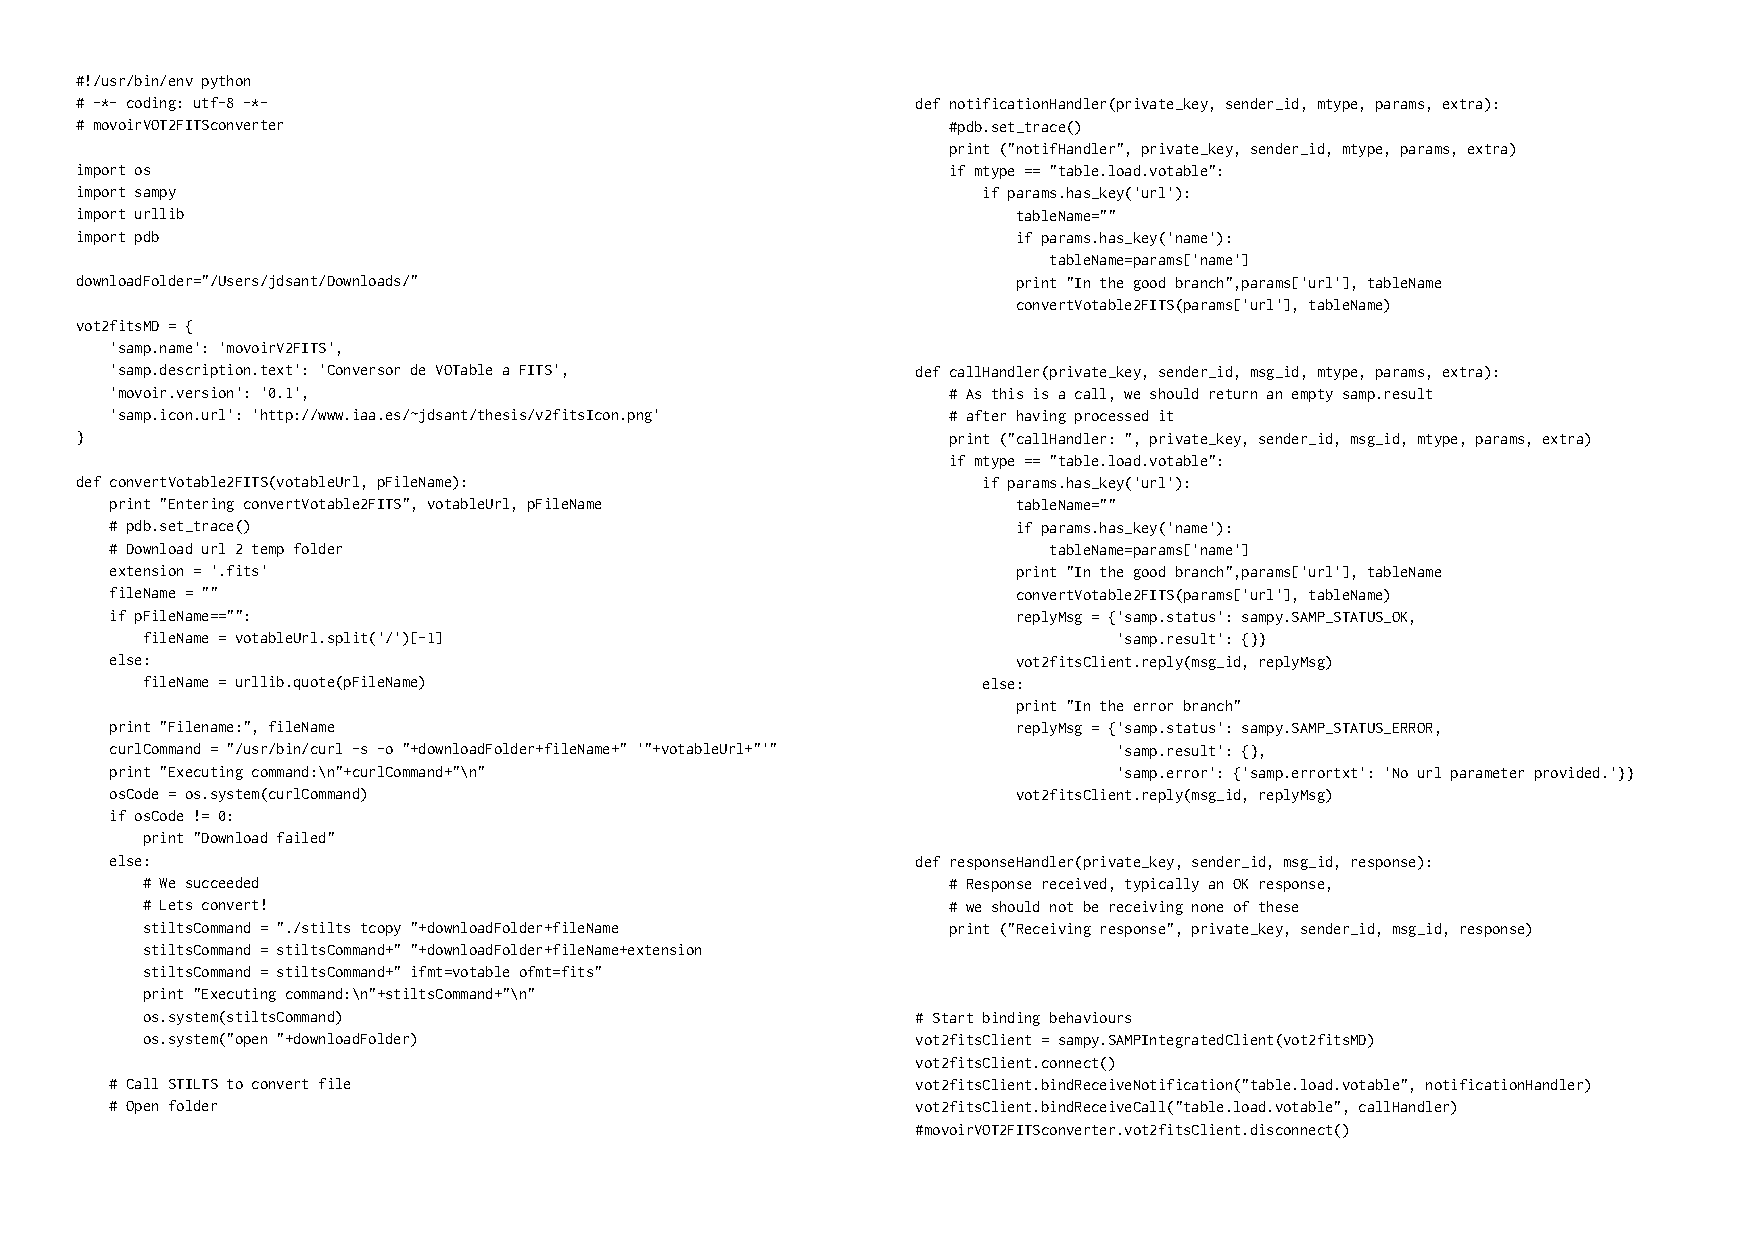
\includegraphics[width=\textwidth]
					{fig/movoirVOT2FITSconvert.pdf}
				\caption[Listing of
				\method{movoirVOT2FITSconverter.py}]
				{Complete listing of
				\method{movoirVOT2FITSconverter.py}.}
				\label{fig:fig_movoirVOT2FITSconvert}
			\end{figure}
			
			The complete listing of the Votable to FITS converter
			module is shown in
			figure~\ref{fig:fig_movoirVOT2FITSconvert}.
			
			Taking into account that the \method{table.load.votable}
			message can be sent both as a notification (specially when
			broadcasted), or as a call (synchronous or asynchronous),
			the module needs to be able to receive that message in any
			of those two flavours.
			
			That is achieved by means of a single processing function,
			\method{con\-vert\-Vo\-ta\-ble\-2\-FITS}, which is called
			from the handlers for notifications or calls.
			
			The last part of the \method{movoirVOT2FITSconvert} module
			is, in fact, the part that it is executed first. It starts
			with the declaration of metadata and the the registration
			of the module with the hub. Later, the calls and
			notifications to the
			\method{table.load.votable} message are bound,
			respectively, to the \method{callHandler}  and
			\method{notificationHandler} functions, respectively.
			
			The handler functions perform a sanity check of the called
			parameters, such as ensuring that the message is indeed a
			\method{table.load.votable} message, and that it provides
			the mandatory \mapkey{url} parameter. Once this is
			ensured, the control is passed to the
			\method{convertVotable2FITS} function, which performs
			the actual conversion.
			
			\method{convertVotable2FITS} is straightforward:
			the
			file name is obtained from the URL, a \method{curl} call
			for data download is setup first, preparing next the
			\method{stilts} call. Once setup, they are called 
			sequentially. Finally, the \method{open} call is used
			\footnote{The \method{open} command is specific to Mac OS
			X; an alternative in Linux, with the Gnome desktop
			installed, is the
			\method{gnome-open} command.} to open the conversion
			folder and reveal both the original and converted files.
			
			The only meaningful difference between the
			movoirVOT2FITSconvert and movoirVOT2CSVconvert modules
			is the output parameter sent the \method{stilts} command,
			and the file extension.
					
		% subsection implementation_details_vodc (end)
	
	% section vo_data_converter (end)
	
	\section{ConeSearcher} % (fold)
	\label{sec:amiga_conesearch}
		
		The ConeSearcher module is a very straightforward,
		Python-based module, which sends a \method{table.load.votable}
		message back with the results of a ConeSearch around a region
		of the sky where the user clicked in applications
		such as Aladin, which send a \method{coord.pointAt.sky}
		MType.
		
		Given that the ConeSearch URL can be built by concatenating
		the archive endpoint, and the
		parameters \mapkey{RA}, \mapkey{DEC}, and \mapkey{SR}, it is
		fairly easy to write the \method{table.load.votable} message
		in response to the \method{coord.pointAt.sky} message.
		
		\subsection{Implementation details} % (fold)
		\label{sub:implementation_details_amigacones}
			
			\begin{figure}[tbp]
				\centering
					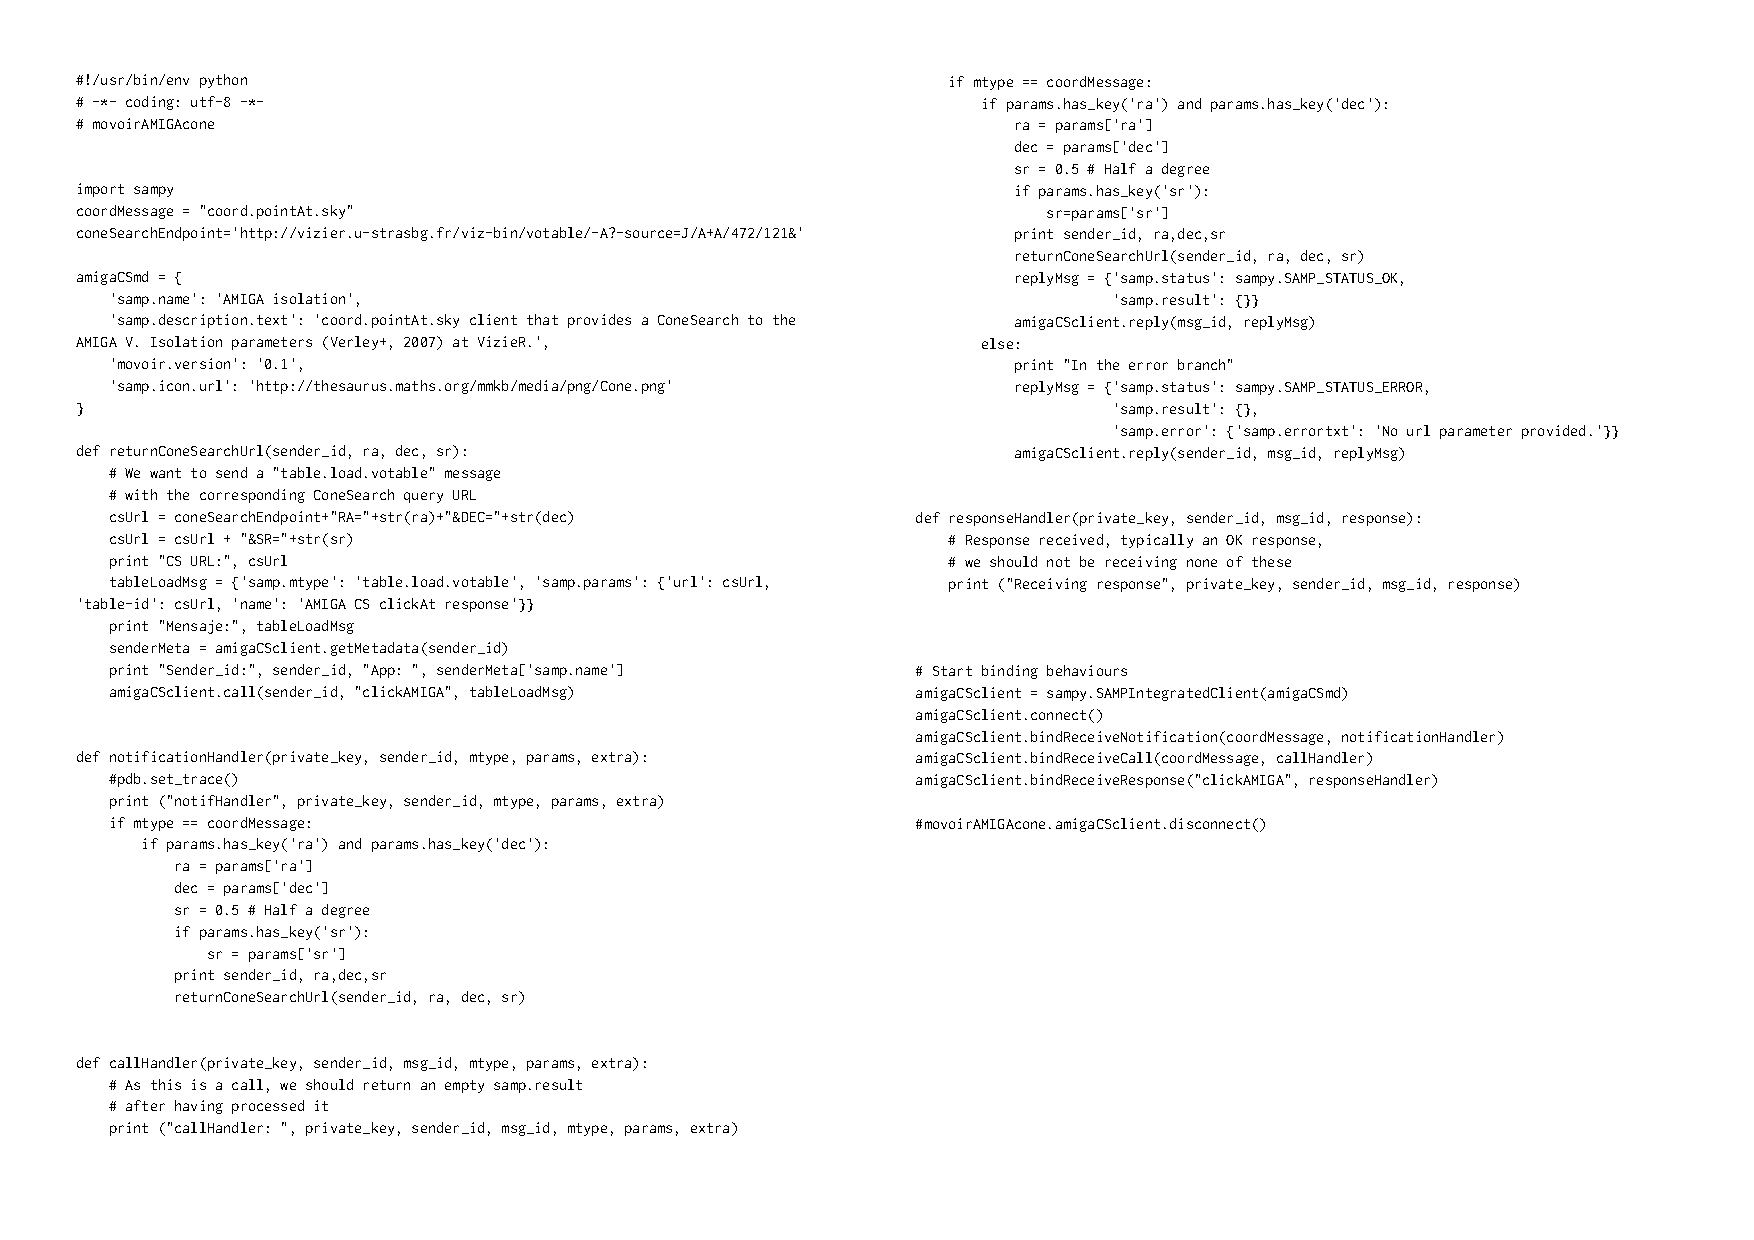
\includegraphics[width=\textwidth]
					{fig/movoirAMIGAcone.pdf}
				\caption[Listing of
				\method{movoirAMIGAcone.py}]
				{Complete listing of
				\method{movoirAMIGAcone.py}.}
				\label{fig:fig_movoirAMIGAcone}
			\end{figure}
			
			
			Figure~\ref{fig:fig_movoirAMIGAcone} shows the
			complete listing for a ConeSearch client based upon
			the \method{coord.pointAt.sky} message and corresponding
			coordinates. In this case, we use the ConeSearch endpoint
			for the AMIGA catalogue of isolation parameters held at
			VizieR.
			
			As this implementation is very similar to the VO Data
			Converter modules, we will just point out that the
			key is the \method{returnConeSearchUrl}, which creates
			the URL to send back via the \method{table.load.votable}
			message, and takes care of providing a suitable name for
			the new table.
			
			\begin{figure}[tbp]
				\centering
					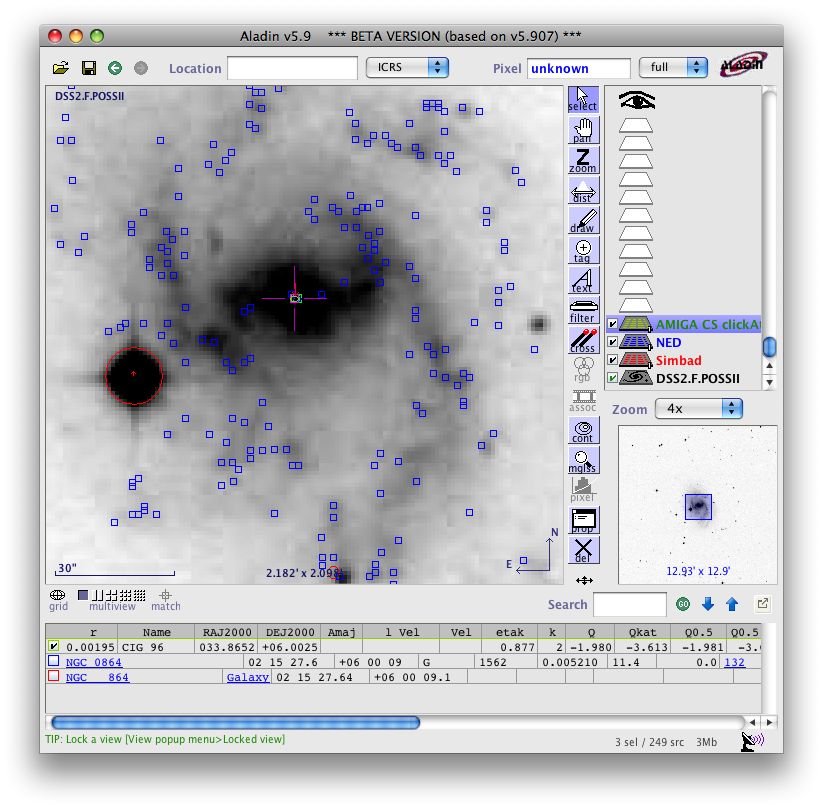
\includegraphics[width=\textwidth]
					{fig/AladinAMIGAcone.png}
				\caption[Aladin showing the MOVOIR ConeSearch module]
				{Aladin Sky Atlas showing the result of having clicked
				near NGC~804, which is one of the galaxies in the
				AMIGA sample, while the MOVOIR ConeSearch module is
				active.}
				\label{fig:fig_AladinAMIGAcone}
			\end{figure}
			
			Figure~\ref{fig:fig_AladinAMIGAcone} shows a screen
			capture of the Aladin Sky Atlas displaying NGC~804, which
			is one of the members of the AMIGA sample of isolated
			galaxies\footnote{Also known as CIG~96, or K73~96}.
			Over the optical image, Aladin is overlaying data from NED
			(blue marks) and Simbad (red marks), but we can also see
			another layer in light green, AMIGA CS clickAt, which has
			been generated from a ConeSearch activated by a click on
			Aladin, which in turn generates the
			\method{coord.pointAt.sky}, which activates the
			ConeSearcher module.
			
			It is trivial to update the module to perform ConeSearches
			in arbitrary endpoints, and indeed it would be
			straightforward to update the module in order to
			incorporate the \method{movoir.configuration.set}
			message, in order to set, for instance, a different
			endpoint, or a different default search radius.
			
			Other trivial uses of \method{coord.pointAt.sky} listeners
			which provide \method{table.load.votable} messages as a
			result would include synthesising the answers from
			different ConeSearches (which can be performed in
			different threads to minimise wait time).
			
			More sophisticated uses can be the development of scripts
			which directly query large survey's databases (for
			instance, SDSS queries using the \method{casjobs} Java
			interface), overlaying the objects (and properties) on a
			certain part of the sky resulting from a given query. Of
			course, once the IVOA Table Access Protocol is finished,
			and compatible services start to appear, including
			remote cross-matching capabilities, the possibilities
			increase significantly.
			
			
		% subsection implementation_details (end)
		
	% section amiga_conesearch (end)
	
	\section{AppleScript XML-RPC SAMP tester} % (fold)
	\label{sec:applescript_xml_rpc_samp_tester}
		
		This is not a proper MOVOIR module. Instead, this is a small
		testing module that was quickly implemented in order to show
		the bare XML-RPC interface of the SAMP protocol (in the
		standard profile).
		
		\begin{figure}[tbp]
			\centering
				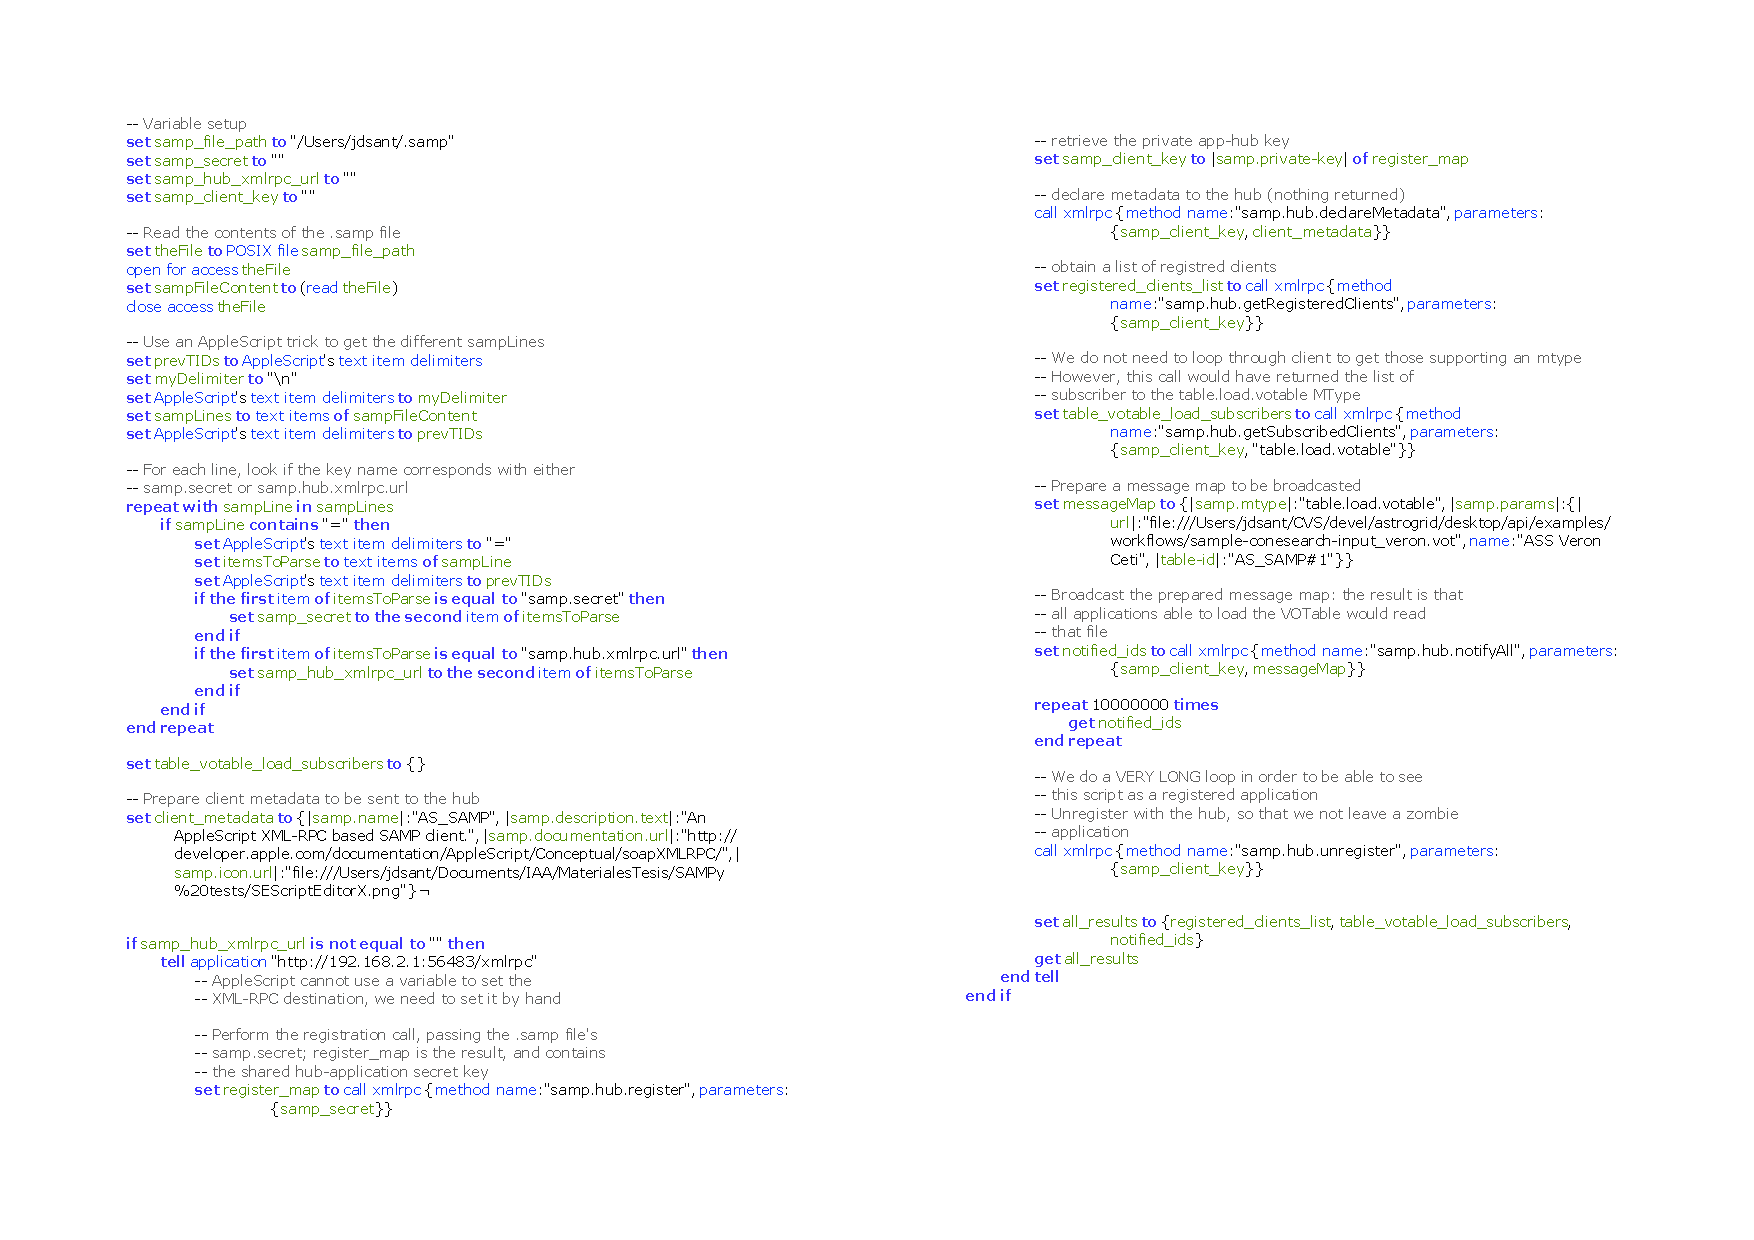
\includegraphics[width=\textwidth]
				{fig/AS_SAMP.pdf}
			\caption[Example AppleScript-based SAMP application]
			{
				Example AppleScript-based SAMP application, which
				shows XML-RPC calls for the XML-RPC profile of the
				SAMP protocol. AppleScript keywords are in blue,
				while variable names are set in green, and string
				literals in black. Comments are preceded by two
				dashes (\texttt{-}\texttt{-}). Source code
				available at:
			\url{http://www.iaa.es/~jdsant/thesis/SAMP.applescript}
			}
			\label{fig:fig_AS_SAMP}
		\end{figure}
		
		Figure~\ref{fig:fig_AS_SAMP} contains the listing of a
		sample AppleScript client which connects to a SAMP hub,
		collects some information, and sends a
		\method{table.votable.load} message.
		
		In order to do that, the \texttt{.samp} file is found,
		loaded, and parsed in order to
		get the values of the \mapkey{samp.secret} and
		\mapkey{samp.hub.xmlrpc.url} keys, while the
		\textbf{\texttt{tell application}} block performs all
		the XML-RPC communication is held.
		
		The steps performed by this script are: registering with
		the hub, interchanging a secret common to hub and
		application; declare the application metadata; getting a
		list of all clients registered with the hub; getting a
		list of all clients subscribed to
		\mapkey{table.load.votable}; create and broadcast a
		\mapkey{table.load.votable} to a local VOTable; remain
		
		Even without knowledge of AppleScript, this example
		illustrates the fact that SAMP messages are
		indeed pure XML-RPC messages, where parameters are sent
		by order, but that limitation can be overcome by using
		maps for setting named parameters, as SAMP does.
		It is also interesting to
		compare figures~\ref{fig:fig_AS_SAMP} and
		\ref{fig:fig_VODownloader_initSamp}, in order to appreciate
		the much higher level of abstraction provided by the JSAMP
		library.
		
		Figure~\ref{fig:fig_AS_SAMP_hub}
		is a screen capture of the SAMP Hub Monitor screen,
		showing the AS\_SAMP registered with the hub and selected,
		in order to see AS\_SAMP metadata.
		
		\begin{figure}[tbp]
			\centering
				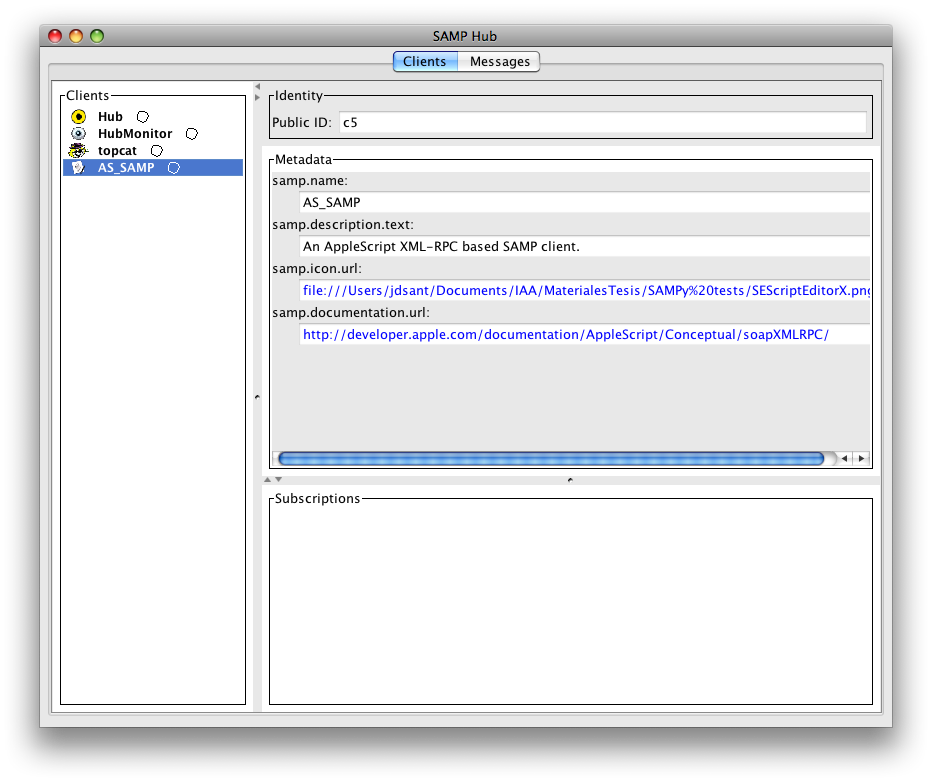
\includegraphics[height=0.4\textheight]
				{fig/AS_SAMP_hub.png}
			\caption[AS\_SAMP AppleScript client]
			{
				Screen capture of the SAMP Hub Monitor showing the
				active applications, and the metadata stored in the hub
				regarding the AS\_SAMP application.
			}
			\label{fig:fig_AS_SAMP_hub}
		\end{figure}
		
		
	% section applescript_xml_rpc_samp_tester (end)
	
	% section bringing_massa_into_the_vo (fold)
	\section{Bringing \massa{} into the VO}
	\label{sec:bringing_massa_into_the_vo}
		
		The modules described in the previous
		sections have been implemented
		in order to be able to bring VO utilities to legacy
		applications without access to application source code.
		Apart from the facilities already implemented by those
		modules, the VO Data Converter module
		---see section~\ref{sec:vo_data_converter}--- illustrates
		how to launch command-line applications after having
		received a SAMP message. We can, therefore, create SAMP
		wrappers for different VO messages. We can easily imagine
		that a mixture between the VO~Downloader (to retrieve the
		remote data, and to launch a command-line application), and
		the VO Data Converter (to convert it into a format suitable
		to the application), can enable the VO-awareness of
		existing applications, by launching it with the received,
		copied, and possibly converted file as a
		parameter\footnote{Besides, several operating systems, such
		as FreeBSD or Mac OS X, provide facilities for detecting
		changes in folder content, so that a script can be launched
		upon change, which opens the possibility of creating SAMP
		messages in order to send data created in particular
		folders to applications of interest.}.
		
		In the case of \massa{}, being a spectral analysis and
		transformation application, the modules should provide
		support for the \method{table.load.votable},
		\method{table.load.fits} ---for spectra expressed as
		tables---, as some of them are, and the more specific
		\method{spectrum.load.ssa-generic}.
		
		However, if there is access to the source code, as is the
		case with \massa{}, it is much more advisable to
		include SAMP support in the application itself.
		
		\begin{figure}[tbp]
			\centering
				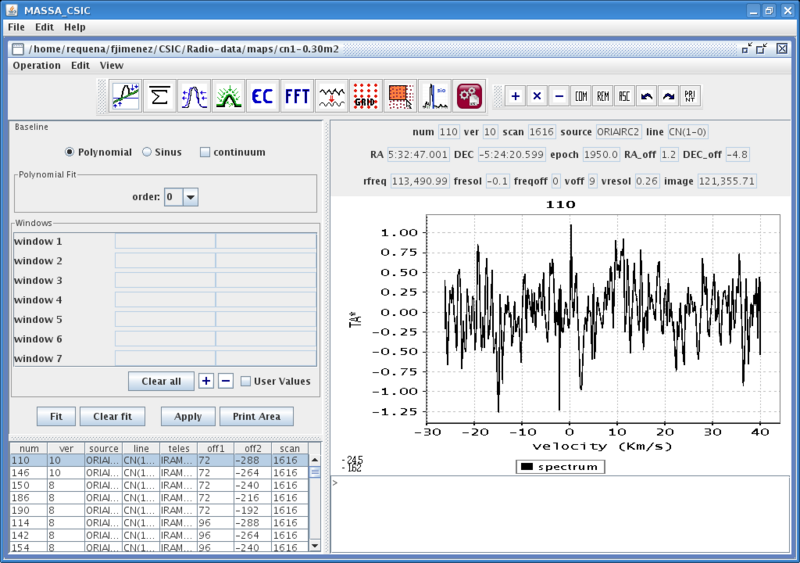
\includegraphics[height=0.4\textheight]{fig/massa1.png}
			\caption[Screen capture of \massa{}]
			{Screen capture of \massa{}.}
			\label{fig:fig_massa1}
		\end{figure}
		
		
		The source code for both \massa{} and
		\madcuba{}\footnote{\madcuba{} is a data cube viewer
		integrated in the same codebase as \massa{}, so that
		\massa{} can build, via a regridding algorithm, datacubes
		from irregularly sampled On-The-Fly observations to be
		later visualised with \madcuba{}.} is composed of 724 Java
		classes, and there are 159 additional files shared between
		HTML documention, JPG images, PNG icons, and test
		\mapkey{.fits} and \mapkey{.30m} files. By concentrating in
		using SAMP in order to enable VO compatibility, we just
		need to touch a few of them. Figure~\ref{fig:fig_massa1}
		shows a screen capture of \massa{}, with one spectrum
		selected among a set of observations.
		
		In particular, and recalling both
	section~\ref{sec:implementing_samp_into_an_existing_application},
		and the introduction of SAMP capabilities into the
		Java-based VO~Downloader, we can see that the candidate
		classes to be changed are just a few.
		
		In particular, we need to:
		
		\begin{itemize}
			\item Include SAMP initialisation after GUI
			initialisation.
			
			\item Include SAMP shutdown at the first stages
			of GUI shutdown.
			
			\item Create \method{*.load.*} handlers which
			make use of existing data creation mechanisms;
			in some cases (VOTables) they will need to
			change format.
			
			\item Create additional menu options for
			sending \massa{} spectra to other VO applications,
			including the creation of VO metadata from the \massa{}
			internal model.
		\end{itemize}
		
		\subsection{Initialising SAMP} % (fold)
		\label{sub:initialising_samp_in_massa}
			
			In \massa{}, the GUI is initialised by the
			\method{initGUI()} method in the \method{MainApp}
			class, which holds the \method{main()} function for
			\massa{}.
			
			 As \method{initGUI()} is called in the
			\method{MainApp} class creator, we will call our
			\initSamp{} method right afterwards, residing in the
			same \method{MainApp} class.
			
			 In it, we will call a single handler functions for the
			different \method{*.load.*} methods. That function will
			call different procedures depending on the actual MType
			being received.
			
			 Figure~\ref{fig:fig_massaVOinHub} shows a screen
			capture of the JSAMP HubRunner with \massa{} registered
			with the hub, metadata declared, and message handlers
			installed.
			
			\begin{figure}[tbp]
				\centering
					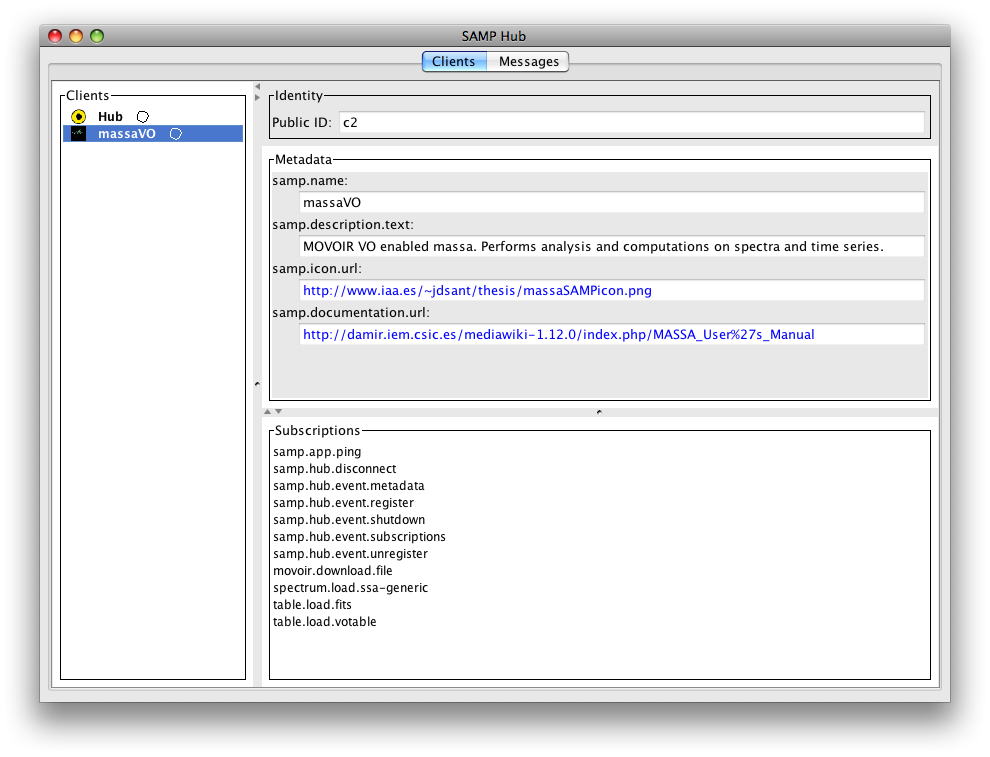
\includegraphics[height=0.4\textheight]
					{fig/massaVOinHub.png}
				\caption{\massa{} registered with the JSAMP Hub}
				\label{fig:fig_massaVOinHub}
			\end{figure}
			
		% subsection initialising_samp_in_massa (end)
		
		\subsection{Shutting down SAMP} % (fold)
		\label{sub:include_samp_shutdown}
			
			To shut SAMP down, we will choose the exit handler
			for \massa{} as the place to install a
			\shutdownSamp{} method. By using the
			\method{JFrame} class as the base class for
			\method{MainApp}, setting up auto-quit on close,
			and having no other quit mechanism, the place
			to install the \shutdownSamp{} method is
			right after having confirmed that indeed we wish to
			close \massa{}.
			
			That way, \massa{} will always correctly unregister
			with the hub on quit.
			
			Once chosen the right place to install the
			\shutdownSamp{} method, the method itself
			is quite simple, and is identical to the one
			used for the VO~Downloader.
			
		% subsection include_samp_shutdown (end)
		
		\subsection{Creating data load handlers} % (fold)
		\label{sub:creating_data_load_handlers}
			
			The simplest data load handler to be created in
			\initSamp{} could just use \massa's \method{Loader} class,
			bypassing the file chooser, and providing directly a
			path to the \method{loadFile} method in that class.
			
			By doing that, however, one of the file types which
			can be understood by \massa's \method{SpectraLoaderFactory}
			class must be provided. Hence, for \method{table.load.fits}
			messages, if the URL sent corresponds to one of the
			FITS file formats understood by \massa, that  would
			be the most straightforward way to implement it.
			
			For \method{table.load.votable} messages, either a
			linked FITS file can be passed to the already
			mentioned \method{loadFile} method, or the VOTable
			can be converted to FITS using a Java library
			such as STIL (the software library which is the
			foundation for the \method{stilts} command), and
			later to the internal model of the application.
			For \method{spectrum.load.ssa-generic} messages
			the URL parameter would point to either an XML
			serialisation of the spectrum or, most likely,
			to a FITS file, making this approach the easiest.
			
			However, and specially for the recently incorporated
			\method{spectrum.load.ssa-generic} message, this
			would completely ignore the associated \mapkey{meta}
			keyword, which corresponds to a map of Spectrum data
			model UTypes as keys.
			
			The alternative is to modify the
			\method{SpectraLoaderFactory}, so that it is provided
			which a special VOTable, created on the fly by the
			\method{*.load.*} method handlers, and which handles
			by itself the creation and configuration of a FITS
			file containing all metadata provided in the
			original message.
			
			In this way, we just modify one class, the
			\method{SpectraLoaderFactory}, create a few more
			classes for handling each different case, and the
			creation of internal structures is left untouched,
			and being able to survive future changes in the
			application internal data model.
			
			\begin{figure}[tbp]
				\centering
					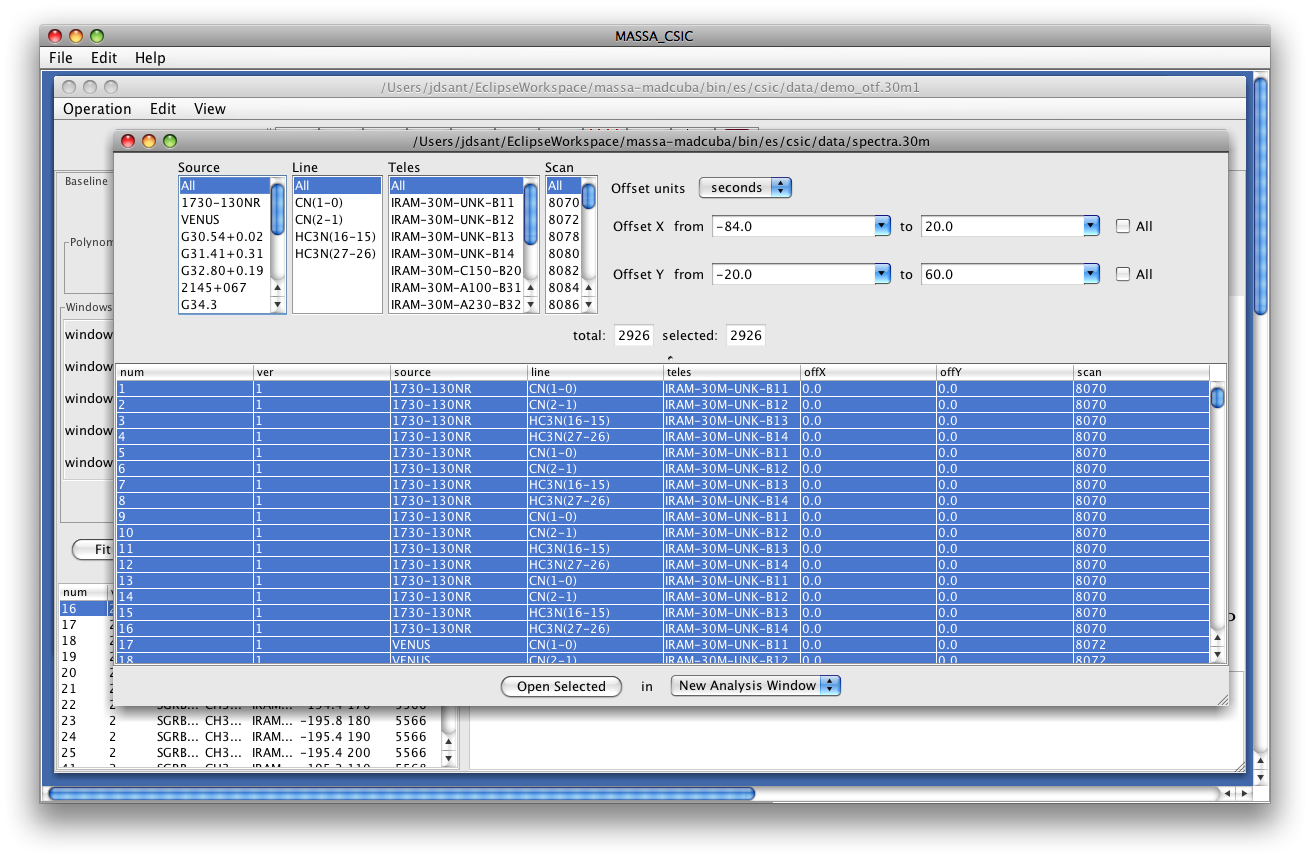
\includegraphics[height=0.4\textheight]
					{fig/massaSelectionWindow.png}
				\caption[\massa's data selection window]
				{\massa showing its data selection window,
				which opens right after having opened a file
				which contains multiple spectra.}
				\label{fig:fig_massaSelectionWindow}
			\end{figure}
			
			The main issue with this approach is that, by the
			way \massa{} is designed, incoming data would be
			shown first in one of \massa's data selection
			windows, such as the one displayed in
			figure~\ref{fig:fig_massaSelectionWindow}. That
			is not a problem per se, but it reduces somehow
			the interactivity with other applications. On the
			other hand, it allows a first peek to the metadata
			of the spectra being received (even if it consist
			of just one spectrum).
			
		% subsection creating_data_load_handlers (end)
		
		\subsection{Adding SAMP menu options} % (fold)
		\label{sub:adding_samp_menu_options}
			
			For \massa{}, the easiest way to introduce SAMP
			data sending menu options would seem to add them to
			the global menu bar, in an Interop menu, mimicking
			the way the SAMP interface is built on applications
			like TOPCAT.
			
			This is, however, not advised, because as
			shown in figure~\ref{fig:fig_massa1}, and glimpsed
			in figure~\ref{fig:fig_massaSelectionWindow}, there
			are different kinds of \massa{} windows, each one
			with its own menu.
			
			We believe that, in the case of \massa{}, it is
			more sensible to provide selection based, context
			sensitive pop-up menus to provide options to:
			
				\begin{itemize}
					\item broadcast the selected spectra
					as a series of \method{spectrum.load.ssa-generic},
					\method{table.load.fits}, or
					\method{table.load.votable} messages;
					
					\item send the selected spectra to particular
					applications; applications supporting
					\method{spectrum.load.ssa-generic} will be
					shown first, with applications supporting
					\method{table.load.fits} next, and those
					supporting \method{table.load.votable} last;
					the sending method would be chosen accordingly,
					and data conversions will be performed as
					needed from the \method{SimpleSpectraBunch}
					internal format.
				\end{itemize}
			
			
		% subsection adding_samp_menu_options (end)
		
	% section bringing_massa_into_the_vo (end)
	
	\section{Conclusions} % (fold)
	\label{sec:movoir_app_conclusions}
		
		By developing a SAMP-based approach for the MOVOIR, we
		have been able to VO-enable \massa{} with minimal
		changes, and at the same time we have provided a mechanism
		for enhancing not only \massa{}, but any other existing
		SAMP-enabled application which is able to send and receive
		standard MTypes.
		
		The lowest common denominator degree of VO compatibility is
		provided by the VO~Downloader, which enables other VO
		applications to send \method{table.load.votable}, or
		\method{image.load.fits} messages, and consolidate those
		files into a folder were legacy applications can retrieve
		useful data; and the VO Data Converters, which are capable
		of providing FITS or CSV files created from VOTables sent
		to them.
		
		We have also shown, however, than if source code is
		available, and there are SAMP libraries for the language and
		platform the legacy application is running on, that the amount
		of code which has to be modified is minimum: code has to be
		added to initialise the SAMP messaging, and SAMP event
		handling, but that is achieved by just adding a single method
		call in the application initialisation, and the shutdown of
		SAMP messaging as the first method in the \method{actionExit}
		method handler.
		
		The only remaining issue to be solved, which is also limited
		to the classes performing data loads, is how to perform the
		adaptation of the FITS or VOTable data files to the internal
		structure of the application.
		
		In the case of VOTables whose role is to describe a FITS file
		whose link is included, the data load handlers only need to
		access that FITS file, and use the regular FITS load
		capabilities included with the application. Finally, sending
		data to other applications needs the prerequisite of installing
		appropriate interface elements, with their corresponding
		\method{actionListeners}, which create a temporary VOTable/FITS
		file from the selected element, or a VOTable with links to
		FITS files for various elements, and send the appropriate
		kind of message.
		
		By being so surgical in our approach to bringing VO
		capabilities to applications, we can ensure that an application
		which has been upgraded to use SAMP can evolve during time, and
		be refactored, and most changes in the SAMP-related modules
		will be restricted to the interface for creating datasets and
		sending datasets in the application, while the rest of the 
		SAMP support code ---SAMP startup and shutdown--- will need
		no changes, unless support for additional messages is
		required by application evolution.
		
	% section conclusions (end)
	
% chapter massa_and_movoir (end)